% ----------------------------------------------------------
\chapter{Comportamento Mecânico de Túneis}
% ----------------------------------------------------------

\section{Influência da escavação e o conceito de convergência da seção}

De uma forma geral, do ponto de vista do maciço, a escavação de um túnel nada mais é do que uma perturbação no seu estado natural de equilíbrio devido à remoção de parte do maciço. Essa perturbação induzirá o maciço a uma nova configuração de equilíbrio que mobilizará tensões tangenciais desviando, dessa forma, a direção das tensões principais no entorno da escavação. Através desse \textbf{arqueamento das tensões}, o próprio maciço participa da sustentação da cavidade. Esse arqueamento pode ser decomposto em dois arcos longitudinais (contidos nos planos horizontal e vertical) e um arco transversal (no plano perpendicular ao eixo do túnel), tal como mostrado na \autoref{arqueamento}.

\begin{figure}[H]
	\begin{center}
		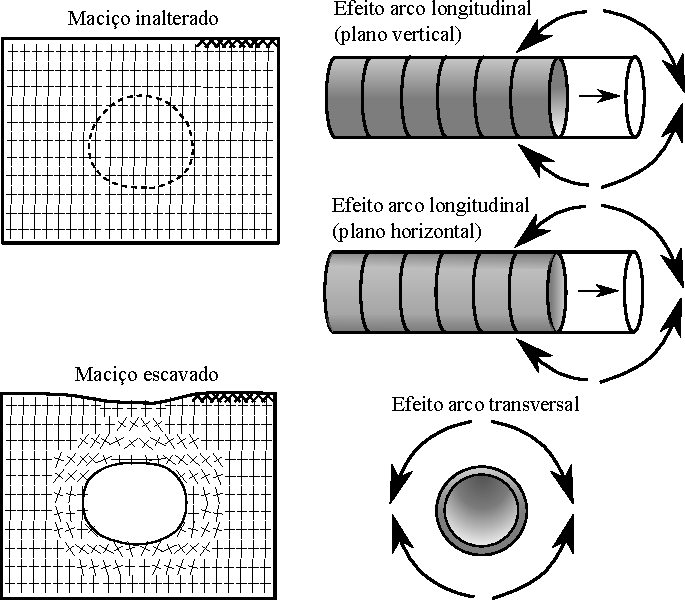
\includegraphics[scale = 1]{0401-efeito_arco.pdf}
	\end{center}
	\caption{\label{arqueamento}Ilustração do arqueamento das tensões principais (adaptado de: \citeonline[p. 10-11]{Franca2006})}
\end{figure}

A presença dos três arcos na zona que acompanha a frente de escavação faz com que essa região tenha um campo de deslocamentos tridimensional convergente em direção à face de escavação. No entanto, conforme essa frente avança e se afasta, apenas o arqueamento transversal se mantém, fazendo com que o campo de deslocamentos seja bidimensional contido no plano transversal ao eixo do túnel. Em vista disso, é conveniente caracterizar três zonas no interior do maciço: uma zona não perturbada pela escavação, uma zona de influência da frente de escavação e uma zona fora dessa influência (\autoref{campo_frente_escavacao}).

\begin{figure}[H]
	\begin{center}
		\includegraphics[scale = 1]{0402-campo vetorial de deslocamentos no maciço.pdf}
	\end{center}
	\caption{\label{campo_frente_escavacao}Campo vetorial de deslocamentos no maciço durante a escavação de um túnel (adaptado de: \citeonline[p. 12]{Franca2006})}
\end{figure}

O parâmetro geométrico mais simples e representativo do comportamento de um túnel é o fechamento de sua cavidade, também conhecido como \textbf{convergência}. Se um túnel circular estiver em um maciço homogêneo, isotrópico, submetido a um estado de tensões inicial geostático hidrostático, o campo de deslocamentos no entorno de uma seção fora da zona de influência da frente de escavação estará contido no plano transversal e será puramente radial, podendo ser expresso por uma função  $u(r)$. Nesse caso, a convergência $U$ é definida pela razão entre o deslocamento da cavidade e seu raio inicial $U=-u(r=R)/R$. A presença do sinal negativo é opcional e serve para que a convergência fique positiva se a seção diminuir, ou seja, $u(R) < 0$  (\autoref{definicao_convergencia}).

\begin{figure}[H]
	\begin{center}
		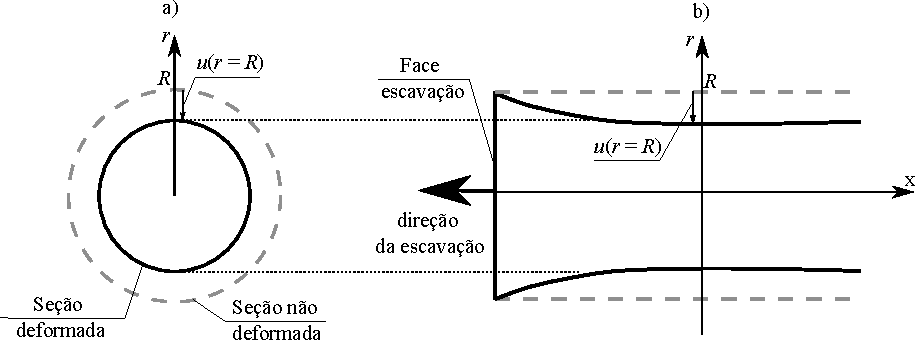
\includegraphics[scale = 1]{0403-convergencia de uma seção circular.pdf}
	\end{center}
	\caption{\label{definicao_convergencia}Ilustração das medidas geométricas que compõe a convergência de uma seção circular: a) corte transversal, b) corte longitudinal}
\end{figure}

Dependendo da anisotropia das tensões \textit{in situ} ou do formato da seção, sua deformada pode não ser radial e, na prática, podem-se usar varias medidas para compor o cálculo da convergência da seção, como exemplificado na \autoref{convergenca_secao_qualquer}.

\begin{figure}[H]
	\begin{center}
		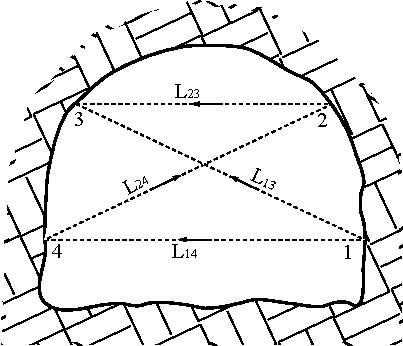
\includegraphics[scale = 1]{0404-convergencia de uma seção qualquer.pdf}
	\end{center}
	\caption{\label{convergenca_secao_qualquer}Medidas da convergência em quatro direções de uma seção não circular (adaptado de: \citeonline[p. 8]{Panet1995})}
\end{figure}

Outro aspecto importante para determinar a influência da escavação e caracterizar o comportamento global do túnel é a representação gráfica das convergências ao longo do seu eixo longitudinal, conhecida como \textbf{perfil de convergências}. Por exemplo, com o objetivo de quantificar a extensão da zona de influência da frente da escavação, Hanafy \& Emery (1980) graficaram o perfil de convergências do seu modelo de um túnel circular em um maciço homogêneo, isotrópico e elástico linear (\autoref{perfil_exemplo}).

\begin{figure}[H]
	\begin{center}
		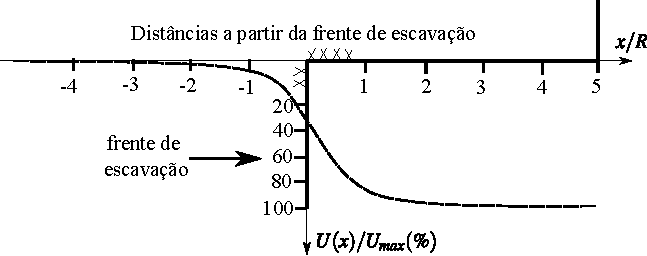
\includegraphics[scale = 1]{0405-perfil de convergencias próximo a frente de escavação.pdf}
	\end{center}
	\caption{\label{perfil_exemplo}Perfil de convergências próximo à frente de escavação (adaptado de: \citeonline{Hanafy1980} \textit{apud} \citeonline[p. 42]{Couto2011})}
\end{figure}

Como se pode ver na \autoref{perfil_exemplo}, dentro das hipóteses dos autores, a partir de cinco raios da face de escavação a convergência atinge seu valor máximo  $U_{max}$. Já na face, em $x/R=0$ , a convergência é superior à 35\% do valor máximo, sendo que a um raio de distância a convergência é de aproximadamente 80\% da total e quase 100\% se tiver ultrapassado dois raios (\citeonline{Hanafy1980} \textit{apud} \citeonline[p. 42]{Couto2011}).

\section{Mecanismos de ruptura em túneis profundos}

A execução de túneis se tornou bastante segura após os preceitos filosóficos e teóricos do método empírico NATM (\textit{New Austrian Tunneling Method}) desenvolvido por Rabcewicz (\citeyear{Rabcewicz1964a}, \citeyear{Rabcewicz1964b} e \citeyear{Rabcewicz1964c}) e \citeonline{Rabcewicz1973}. E cada vez mais os estudos numéricos vêm ajudando os projetistas na tomada de decisões seguras durante a fase de projeto e execução. Contudo, apesar dessa abordagem empírica e numérica ter diminuído significativamente o número de incidentes estes ainda existem. Compilados de acidentes podem ser encontrados em estudos da \citeonline{HealthandSafetyExecutiveHSE1996} e de pesquisadores como \citeonline{Stallmann2005}, \citeonline{Seidenfus2006} e \citeonline{Sousa2010}, tal como reunido por \citeonline{Spackova2012} na \autoref{incidentes}.

\begin{figure}[H]
	\begin{center}
		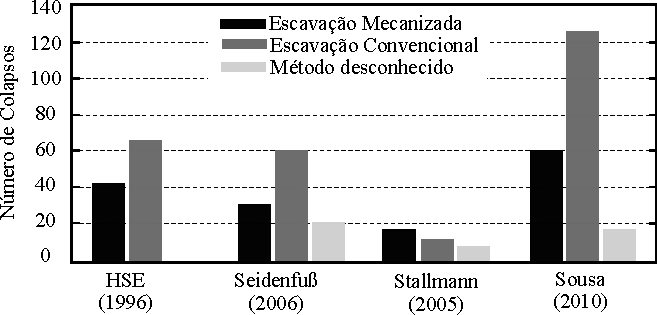
\includegraphics[scale = 1]{0406-número de incidentes em quatro banco de dados descriminado por autor e tecnologia de escavação.pdf}
	\end{center}
	\caption{\label{incidentes}Número de incidentes em quatro banco de dados descriminados por autor e método de escavação (adaptado de: \citeonline[p. 19]{Spackova2012})}
\end{figure}

\citeonline{Sousa2010}, por exemplo, agrupou os incidentes, tanto de túneis profundos como superficiais, em nove tipos, tal como apresentado na \autoref{distribuicao_incidentes}.

\begin{figure}[H]
	\begin{center}
		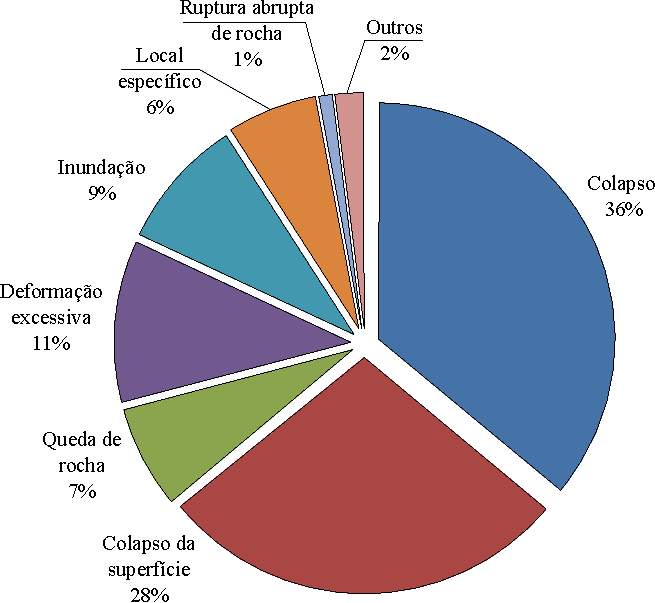
\includegraphics[scale = 1]{0407-distribuição de incidentes de acordo com nove tipologias.pdf}
	\end{center}
	\caption{\label{distribuicao_incidentes}Distribuição de incidentes de acordo com nove tipologias (adaptado de: \citeonline[p. 82]{Sousa2010})}
\end{figure}

Contudo, de forma geral, no comportamento de túneis profundos executados em maciços aparentemente contínuos, ou seja, ausência de grandes descontinuidades ou acidentes geológicos, identifica-se dois mecanismos principais de colapso (ou ruptura): \textit{Spalling} (descamação ou fragmentação) e \textit{Squeezing} (deformações excessivas diferidas no tempo).

O \textit{Spalling} é preponderante em maciço muito resistente, inicialmente pouco fraturado, no qual o nível de energia para iniciar a fissuração e consequente propagação costuma ser alto. Durante a redistribuição das tensões, causada pela escavação, as fissuras vão se desenvolvendo e destacando regiões da rocha no contorno da seção. Essas sofrem então uma descamação, ou ainda, ruptura por flambagem e tem-se, nesse último caso, uma repentina liberação de energia. Uma ruptura abrupta da rocha (\textit{rockburst}). Esse comportamento é refletido na curva tensão-deformação de uma amostra do maciço, por um significativo amolecimento após o pico de resistência, caracterizando, dessa forma, a rocha como frágil \cite[p. 83]{Kleine2007}. A \autoref{mecanismo_spalling} exemplifica esse mecanismo e a \autoref{foto_spalling} mostra a seção após tal colapso.

\begin{figure}[H]
	\begin{center}
		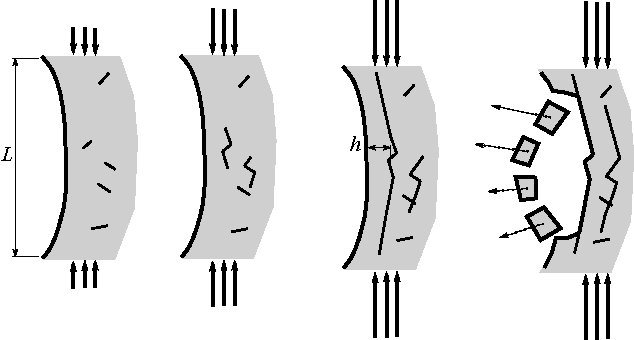
\includegraphics[scale = 1]{0408-mecanismo de ruptura do maciço próximo a seção.pdf}
	\end{center}
	\caption{\label{mecanismo_spalling}Mecanismo de ruptura por \textit{Spalling} de um comprimento $L_s$ junto à seção do túnel: detalhamento do crescimento das fissuras e flambagem de uma profundidade $h_s$ da rocha no contorno da seção (adaptado de: \citeonline[p. 267]{Germanovich2000})}
\end{figure}

\begin{figure}[H]
	\begin{center}
		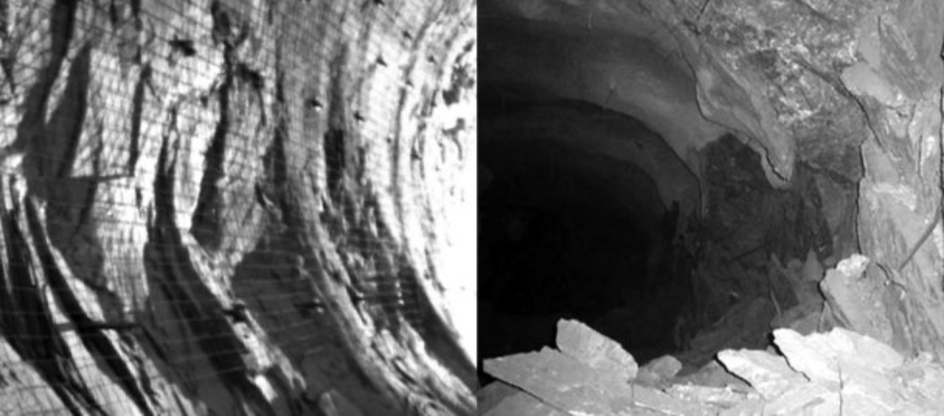
\includegraphics[scale = 1]{0409-foto ruptura por spalling.pdf}
	\end{center}
	\caption{\label{foto_spalling}À esquerda uma seção remanescente após moderada fragmentação e quebra em um túnel escavado com TBM e à direita uma seção em que parte do contorno apresentou instabilidade (flambagem) em um túnel escavado de forma não mecanizada (fonte: \citeonline[p. 1084]{Diederichs2007})}
\end{figure}

Já o \textit{Squeezing} é um modo de falha relacionado ao cisalhamento e encontrado principalmente em túneis profundos em condições de grandes tensões \textit{in situ}. Inicia-se quando a fissuração está suficientemente avançada, causando uma diminuição nas propriedades mecânicas do maciço, sem gerar instabilidade no contorno da seção. Essa diminuição das características mecânicas associada ao desenvolvimento da fissuração é progressiva e controlada, em especial, devido ao confinamento que reina no maciço. Ao contrário do primeiro mecanismo, a energia armazenada pela redistribuição das tensões é dissipada de forma gradual por deformações. Esse comportamento está intimamente relacionado com o fenômeno de fluência descrito na próxima seção a qual compreende um dos comportamentos que se pretende modelar e estudar nessa tese.

A \autoref{evolucao_convergencia} ilustra a evolução da convergência por esse fenômeno. Tal comportamento também é visto em galerias para estocagem de rejeitos radioativos em maciços argilosos profundos. Essas argilas possuem baixa condutividade hidráulica, portanto, pouca difusão molecular, sendo ideais para estocar esse material. Porém, apresentam esse comportamento diferido e que pode comprometer o projeto no longo tempo requerido para estabilização desse material radioativo. Estudos como os de \citeonline{Rousset1988} e \citeonline{Armand2013} são alguns exemplos de investigações nesse sentido. Laboratórios como o HADES na Bélgica e \textit{Meuse/Haute-Marne} (\autoref{evolucao_GED}) em Paris, são exemplos de túneis para estocagem radioativa que apresentam esse fenômeno.

\begin{figure}[H]
	\begin{center}
		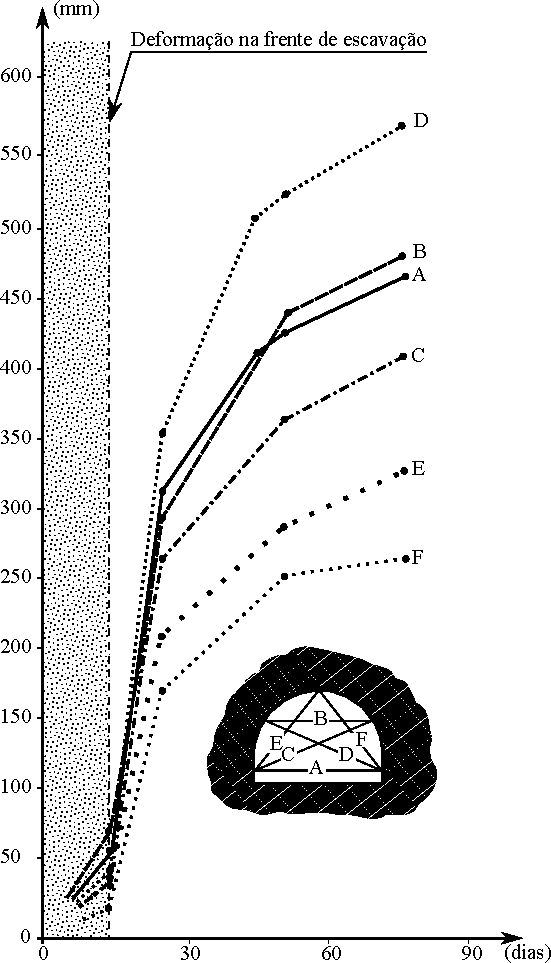
\includegraphics[scale = 1]{0410-evolução da convergencia do túnel fréjus.pdf}
	\end{center}
	\caption{\label{evolucao_convergencia}Evolução da convergência do túnel Fréjus (adaptado de: \citeonline[p. 17]{Lunardi1980})}
\end{figure}

\begin{figure}[H]
	\begin{center}
		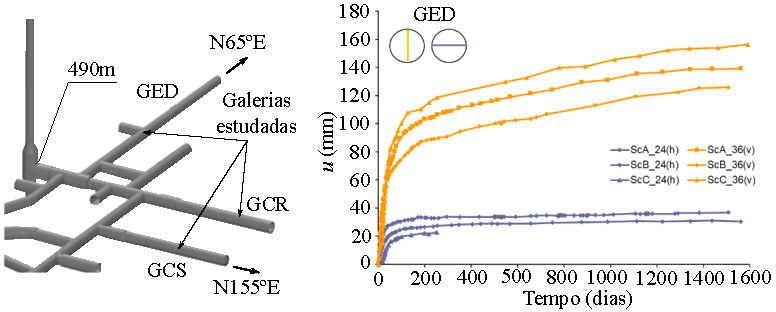
\includegraphics[scale = 1]{0411-evolucação do fechamento da seção C.pdf}
	\end{center}
	\caption{\label{evolucao_GED}Evolução do fechamento da seção GED (convergência) na galeria do laboratório \textit{Meuse/Haute-Marne}  (adaptado de: \citeonline[p. 103]{Guayacan-Carrillo2016})}
\end{figure}



\section{Influência da reologia do maciço}

\subsection{Comportamento instantâneo}

Para caracterizar o comportamento de curto prazo do maciço, o ensaio triaxial associado à medição da variação do volume é comumente utilizado. Esse ensaio clássico na mecânica das rochas permite estudar as diferentes fases do comportamento: elástica, plástica, ruptura e pós ruptura. As medidas da variação do volume permitem fazer estudos de outros aspectos do comportamento, como o coeficiente de Poisson e a dilatância. Esse ensaio, de forma resumida, consiste em submeter uma amostra cilíndrica do maciço a um estado de tensões triaxial hidrostático e, após atingido esse estado, leva-lá à ruptura através do aumento da carga axial (o desviador). \citeonline{Rousset1988}, por exemplo, caracterizou o comportamento de curto prazo de maciços argilosos profundos em frágil (argila rígida) e dúctil (argila plástica). Um maciço rígido pode ser visto na \autoref{ensaio_triaxial_rigido}.

\begin{figure}[H]
	\begin{center}
		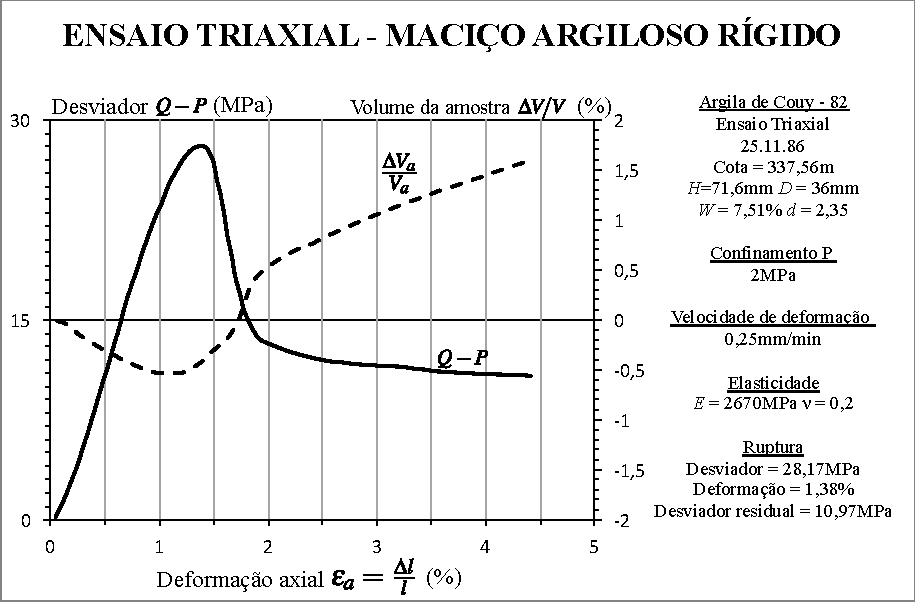
\includegraphics[scale = 0.95]{0412-ensaio triaxial argila rigida.pdf}
	\end{center}
	\caption{\label{ensaio_triaxial_rigido}Ensaio triaxial com medição da variação do volume para o caso de uma argila rígida  (adaptado de: \citeonline[p. 35]{Rousset1988})}
\end{figure}

No comportamento da \autoref{ensaio_triaxial_rigido} pode-se destacar as seguintes fases \cite[p. 34]{Rousset1988}:

\begin{alineas}
	
	\item \textbf{fase elástica} ($0\le \varepsilon_a \le 0,8\%$): o comportamento do maciço é linear elástico e, ao mesmo tempo, o volume da amostra diminui linearmente, os dois parâmetros elásticos, módulo de Young e Poisson, são facilmente obtidos;
	
	\item \textbf{fase pré-ruptua} ($0,8\%\le \varepsilon_a \le 1,3\%$): o desviador continua aumentando, mas a curva $Q-P$ não é mais linear, indicando que fenômenos irreversíveis passam a ocorrer. Ao mesmo tempo, a taxa de redução do volume diminui. Nessa fase também pode-se notar que os fenômenos irreversíveis ocorrem primeiro na curva ${\Delta V}/{V}\;$, em torno de 0,8\% da deformação enquanto o desviador é de 65\% do seu valor máximo e sua dependência ainda é linear;
	
	\item \textbf{fase de ruptura} ($1,3\%\le \varepsilon_a \le 1,6\%$): o desviador cai acentuadamente, o que reflete a fragilidade do comportamento dessa argila. Enquanto isso, o volume da amostra aumenta drasticamente;
	
	\item \textbf{fase pós-ruptura} ($1,6\%\le \varepsilon_a \le 5\%$): o desviador evoluiu pouco e mantém um valor residual de 40\% do desvio máximo. Esta resistência residual ocorre pelo atrito ao deslizamento na superfície de ruptura que apareceu durante o carregamento. Nessa fase, o volume da abertura aumenta muito, o que reflete o comportamento altamente dilatante do material (2\% superior ao volume original na deformação de 5\%).
	
\end{alineas}

Já para um maciço argiloso dúctil, o comportamento é diferente, tal como mostrado na \autoref{ensaio_triaxial_ductil}.

\begin{figure}[H]
	\begin{center}
		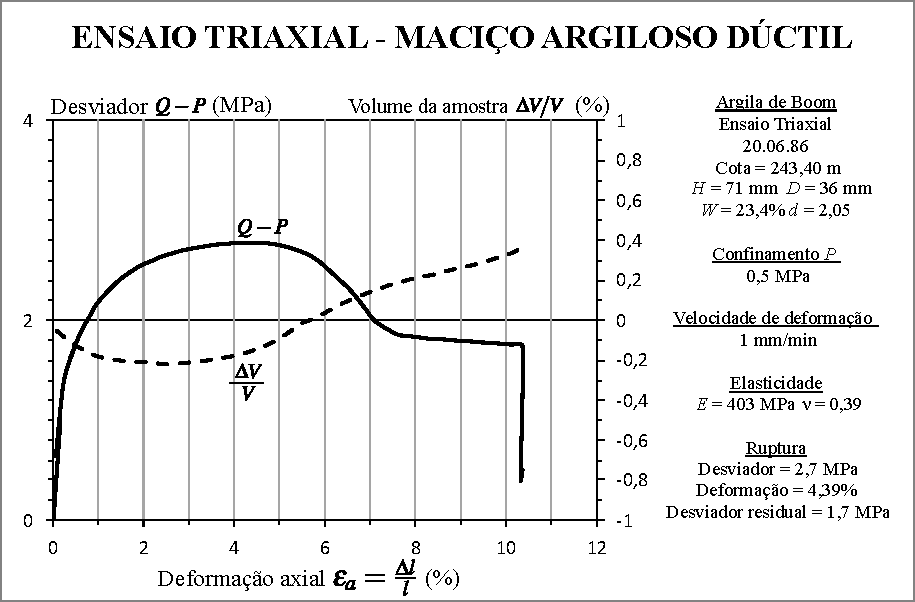
\includegraphics[scale = 0.95]{0413-ensaio triaxial argila ductil.pdf}
	\end{center}
	\caption{\label{ensaio_triaxial_ductil}Ensaio triaxial com medição da variação do volume para o caso de uma argila dúctil (adaptado de: \citeonline[p. 35]{Rousset1988})}
\end{figure}

No comportamento da \autoref{ensaio_triaxial_ductil} pode-se destacar as seguintes fases \cite[p. 35]{Rousset1988}:

\begin{alineas}
	
	\item \textbf{fase elástica} ($0\le \varepsilon_a \le 0,3\%$): pode-se ver que para esse caso, onde ambas as curvas são lineares, é uma fase muito pequena;
	
	\item \textbf{fase plástica com endurecimento} ($0,3\%\le \varepsilon_a \le 2\%$): durante essa fase o desviador continua a aumentar, mas a uma taxa decrescente. Da mesma forma, a redução do volume também teve sua taxa diminuída, mas o comportamento segue ainda de contração;
	
	\item \textbf{fase plástica perfeita} ($2\%\le \varepsilon_a \le 5\%$): o desviador agora segue quase constante e o volume da amostra acompanha o comportamento. Essa fase conduz a uma deformação significativa, superior a 5\%;
	
	\item \textbf{fase plástica com amolecimento} ($5\%\le \varepsilon_a \le 8\%$): a resistência da amostra diminui gradualmente até um platô residual e o volume começa a aumentar;
	
	\item \textbf{fase plástica residual} ($8\%\le \varepsilon_a \le 10\%$): o desviador é agora novamente constante, cerca de 60\% do valor máximo. O volume da amostra aumenta sensivelmente tendo uma dilatância moderada.
	
\end{alineas}

Para um maciço homogêneo, isotrópico e elástico linear a solução analítica para o campo de deslocamentos e tensões no entorno de uma seção circular afastada da zona de influência da face de escavação é conhecida desde \citeonline{Lame1852} e \citeonline{Kirsch1898}, sendo que este último generalizou a solução para um estado de tensões \textit{in situ} anisotrópico. 

Contudo, como visto nas figuras acima, a massa rochosa não é um material perfeitamente elástico e dependendo da magnitude das tensões \textit{in situ} e do desvio das tensões causada pela escavação, o túnel pode apresentar uma zona plastificada ao redor da cavidade. Quando a seção é circular, o maciço homogêneo, isotrópico, elastoplástico, com tensões iniciais geostáticas-hidrostáticas, essa zona plástica é circular e caracterizada por um raio plástico $R^p$. \autoref{deslocamentos_tensoes_analitico} ilustra a solução analítica de um maciço elástico e um elastoplástico. Apesar de a solução depender da forma da lei constitutiva elastoplástica, em geral, para túneis não revestidos, há uma diminuição nas tensões ao redor da cavidade e um aumento na convergência.

\begin{figure}[H]
	\begin{center}
		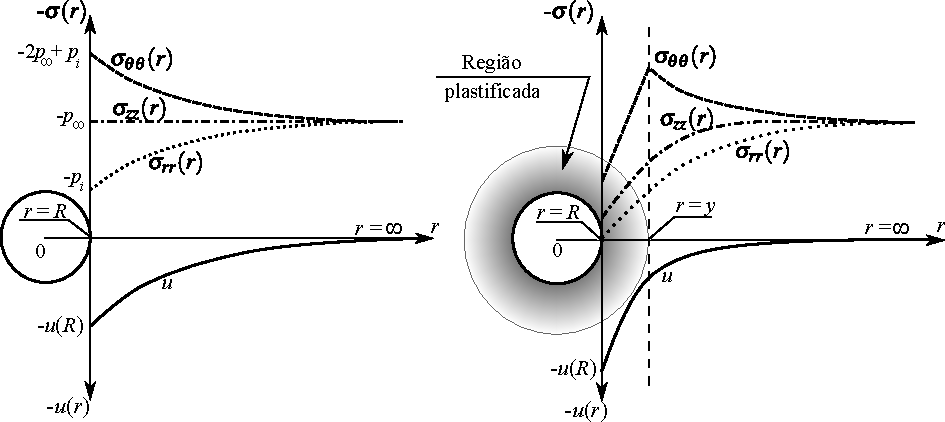
\includegraphics[scale = 1]{0414-campo de deslocamento e tensões no entorno de uma seção circular.pdf}
	\end{center}
	\caption{\label{deslocamentos_tensoes_analitico}Deslocamentos e tensões no entorno de um maciço submetido à pressão geostática-hidrostática $p_{\infty}$ e pressão interna $p_i$ no interior da seção do túnel. À esquerda, maciço elástico e à direita, elastoplástico.}
\end{figure}

Algumas soluções analíticas considerando leis elastoplásticas específicas para túneis não revestidos podem ser encontradas, por exemplo, em \citeonline{Salencon1969}, \citeonline{Hoek1980}, \citeonline{Brown1983}, \citeonline{Detournay1987}, \citeonline{Carranza-Torres1999}, \citeonline{Carranza-Torres2004}, Sharan (\citeyear{Sharan2003,Sharan2005}) e \citeonline{Alejano2009}.

Um dos objetivos desta tese é justamente implementar um algoritmo geral para considerar esse comportamento instantâneo elastoplástico conjuntamente com o fenômeno diferido no tempo.

\subsection{Comportamento diferido no tempo}

O comportamento viscoso do maciço, caracterizado pela deformação contínua no tempo, mesmo sobre tensão e temperatura constantes, é denominado \textbf{fluência} (\textit{Creep}). E ocorre devido aos deslizamentos, quebras e acomodações no interior do maciço e, também, em conjunto com transporte e difusão de massa fluída. Em solos argilosos com condições drenadas, parte da fluência é dada conjuntamente com a dissipação de poro-pressão. Em maciços rochosos, com pouca umidade, essa condição está bastante relacionada com o avanço de trincas e fissuras sobre grande confinamento. Esse comportamento é geralmente caracterizado através de um ensaio triaxial de fluência com uma amostra do maciço. Nesse teste, sobre condições de temperatura e umidade controladas, registram-se as deformações axiais da amostra temporalmente, mantendo-se uma pressão hidrostática e um dado desviador constante. Dessa forma, tem-se a curva típica apresentada na \autoref{curva_caracteristica_fluencia}.

\begin{figure}[H]
	\begin{center}
		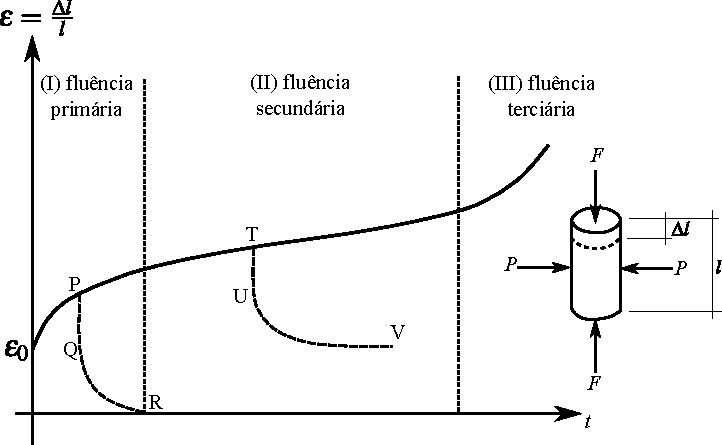
\includegraphics[scale = 1]{0415-curva característica de um ensaio de fluência com os três estágios de comportamento.pdf}
	\end{center}
	\caption{\label{curva_caracteristica_fluencia}Curva característica em um ensaio de fluência com os três estágios de comportamento (adaptado de: \citeonline[p. 107]{Costa1984})}
\end{figure}

Conforme pode-se ver na figura acima, no instante de aplicação da carga axial o corpo de prova sofre uma deformação instantânea inicial $\varepsilon_{a_{0}}$ elástica ou, dependendo do nível das tensões, elastoplástica. Conforme o tempo avança as deformações continuam aumentando, porém, a uma taxa decrescente. Esse estágio é chamado de \textbf{fluência primária} (ou transiente), pois em seguida a taxa de deformação diminui até ficar constante iniciando dessa forma o segundo estágio chamado de \textbf{fluência secundária} (permanente ou estacionária). Após essa fase, que pode consumir a maior parte do tempo, as deformações podem evoluir para o terceiro estágio chamado de \textbf{fluência terciária} (instável), onde a taxa de deformação passa a aumentar até que o material atinge a ruptura \cite{Costa1984}. Contudo, dependendo do nível das tensões, nem sempre a amostra apresenta os três estágios, podendo, inclusive, haver uma estabilização das deformações no tempo.

Além desses estágios de comportamento citados, a recuperação das deformações é outro fenômeno característico de materiais em regime de fluência. Se durante a fluência primária for retirada a carga desviadora o corpo recuperará a sua configuração original seguindo a trajetória $\overline{\textrm{PQR}}$, sendo o trecho $\overline{\textrm{PQ}}$ uma recuperação rápida e instantânea e o trecho $\overline{\textrm{QR}}$ uma recuperação lenta, assintótica e completa (salvo se houverem deformações plásticas durante o carregamento). Nesse caso, em que a recuperação é completa, o maciço está em regime viscoelástico. Contudo, se a descarga for feita no segundo estágio, haverá o mesmo comportamento instantâneo (trecho $\overline{\textrm{TU}}$) e assintótico (trecho $\overline{\textrm{UV}}$), mas a recuperação pode não ser mais completa. Nesse caso, evidencia-se o material comportando-se em seu regime viscoplástico \cite{Costa1984}. Um exemplo típico desse ensaio pode ser visto na \autoref{curva_caracteristica_fluencia_ensaio}.

\begin{figure}[H]
	\begin{center}
		\includegraphics[scale = 1]{0416-ensaio triaxial de fluência da Argila de Boom.pdf}
	\end{center}
	\caption{\label{curva_caracteristica_fluencia_ensaio}Ensaio triaxial de fluência da Argila de Boom (adaptado de: \citeonline[p. 42]{Rousset1988})}
\end{figure}

Na figura acima, pode-se destacar as seguintes fases \cite[p. 42]{Rousset1988}:

\begin{alineas}
	
	\item para um pequeno desviador (1,75MPa) a deformação aumenta rapidamente no início. Sua evolução, em seguida, diminui e se estabiliza depois de alguns dias. Nessa etapa foi observado apenas a fase primária, transiente;
	
	\item para um desviador moderado (2,25MPa), após uma fase rápida, mas desacelerada (fase primária), observa-se o desenvolvimento de uma fase com taxa de deformação constante ($\dot{\varepsilon_a}\simeq 7\cdot {{10}^{-6}}{{h}^{-1}}$). Essa é uma fase de fluência secundária, que leva a deformações relativamente importantes, da ordem de 3,5\% após três meses;
	
	\item para um desviador forte (2,75MPa), próximo do limite máximo de resistência do comportamento instantâneo (\autoref{ensaio_triaxial_ductil}), a taxa de deformação da fase secundária é cinco vezes maior do que a anterior. Após duas semanas, leva a um aumento na taxa de deformação (fase terciária) e, finalmente, a ruptura da amostra, logo que a deformação ultrapassa 6\%.
	
\end{alineas}

Como pode-se ver na \autoref{curva_caracteristica_fluencia_ensaio}, o ensaio de fluência permite conhecer os diferentes limiares que separam os diferentes comportamentos viscosos: fluência primária, secundária, secundária com terciária seguida de ruptura. Também é possível estimar a velocidade das deformações por fluência durante a fase secundária, dependendo da magnitude do desviador. Dessa forma, pode-se obter os principais parâmetros de viscosidade para o modelo do material. Cabe salientar que a fluência depende da interação entre fatores intrínsecos do maciço (como a forma, defeitos e composição da micro e macroestrutura) com fatores extrínsecos (como a magnitude da tensão desviadora, temperatura, pressão de confinamento e umidade). Consequentemente, os ensaios procuram simular esses fatores externos de modo a obter parâmetros mais próximos da realidade para uma correta modelagem. Maiores detalhes sobre ensaios de fluência e caracterização desse comportamento podem ser obtidos em \citeonline{Rousset1988}, para o caso de maciços argilosos profundos ou ainda em \citeonline{Feda1992}, \citeonline{Hunsche1994}, \citeonline{Dusseault1993} e \citeonline{Cristescu1998} para outros diversos casos.

Portanto, no comportamento do túnel, além da deformação instantânea (resultante da redistribuição das tensões e possível plastificação do maciço ao redor da cavidade), deformações diferidas podem ocorrer e, dado a magnitude dos efeitos, pode tender a estabilização ou levar o sistema maciço-revestimento a danos e colapso. De forma ilustrativa, a \autoref{evolucao_U_t_x} mostra a convergência $U$ em função do tempo $t$ e do avanço da escavação $x$ para uma dada seção.

\begin{figure}[H]
	\begin{center}
		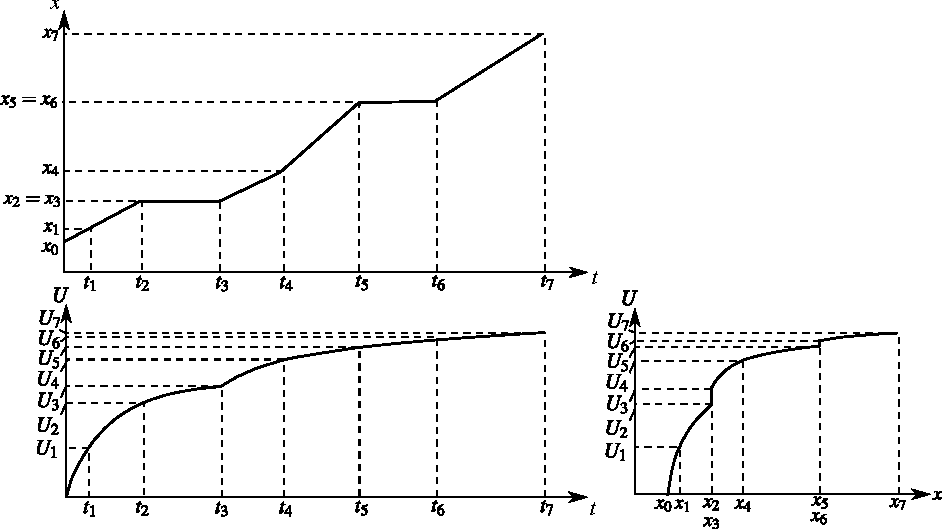
\includegraphics[scale = 1]{0417-evolução da convergência U no tempo t em função do avanço da escavação.pdf}
	\end{center}
	\caption{\label{evolucao_U_t_x}Evolução da convergência $U$ no tempo $t$ em função do avanço da escavação $x$ (adaptado de: \citeonline[p. 12]{Panet1995})}
\end{figure}

Como pode-se ver na figura acima, mesmo sem escavar nos intervalos $[t_2,t_3]$ e $[t_5,t_6]$ a convergência não é constante, tal como seria em um maciço apenas elástico ou elastoplástico. Além disso, nesse caso ilustrativo, a convergência não só evoluiu como também se estabiliza em uma assintótica com o tempo, indicando que a fluência está em um regime primário ou secundário. 

Do ponto de vista da modelagem há diversas formas de introduzir esse comportamento nas análises de túneis, sejam em soluções analíticas ou numéricas, diversas leis constitutivas são empregadas. Podem-se classificar essas leis como: 

\begin{alineas}
	
	\item \textbf{empírico-experimentais}: geralmente são leis expressas por funções ajustadas empiricamente. Para tal existem funções potenciais, como em \citeonline{Obert1965}, exponeciais em \citeonline{Singh1968} e hiperbólicas como em \citeonline{Mesri1981} e \citeonline{Phienwej2007};
	
	\item \textbf{acoplamento hidro-mecânico}: leis que consideram o maciço como sendo constituído por uma fase sólida e fluída. Exemplos dessa abordagem podem ser encontrados nos trabalhos de \citeonline{Griffiths1994}, \citeonline{Leem1999}, \citeonline{Wong2008}, \citeonline{Deleruyelle2014} e \citeonline{Prassetyo2018}.
	
	\item \textbf{Viscoelásticas}: leis formuladas através da analogia com sistemas mecânicos derivados da associação de elementos simples (mola e amortecedor). Estudos com essa abordagem podem ser encontrados em \citeonline{Sakurai1978}, \citeonline{Panet1979}, \citeonline{Sulem1987}, \citeonline{Ladanyi1988}, \citeonline{Goodman1989}, Pan e Dong (\citeyear{Pan1991a}, \citeyear{Pan1991b}), \citeonline{Fahimifar2010}, \citeonline{Wang2014} e \citeonline{Wang2018};
	
	\item \textbf{Viscoplásticas}: leis formuladas através da teoria da plasticidade dependente do tempo, que, tal como as leis viscoelásticas, também possuem uma analogia com sistemas mecânicos elementares, mas introduzem um elemento de atrito, para representar o estado de tensões a partir do qual o fenômeno passa a ter importância. Leis desse tipo podem ser encontradas nos estudos de \citeonline{Berest1983}, \citeonline{Fritz1984}, Cristescu (\citeyear{Cristescu1985}, \citeyear{Cristescu1988}), \citeonline{Ottosen1986}, \citeonline{Bernaud1991}, \citeonline{Gioda1994}, \citeonline{Boidy2002}, \citeonline{Sekine2009} e Roate\c{s}i (\citeyear{Roatesi2012},\citeyear{Roatesi2014}).
	
\end{alineas}

Um exemplo da magnitude dos efeitos viscosos frente a leis elásticas e elastoplásticas em túneis profundos, pode ser vista no perfil de convergências da \autoref{perfil_convergencias_sterpi} obtidas de análises em axissimetria. Quando se considera no modelo apenas a lei elastoviscoplástica em regime secundário, tal possui um comportamento intermediário entre as leis elásticas e elastoplásticas. Além disso, quanto mais rápido a escavação, mais a resposta se aproxima da solução em elasticidade e quanto mais lenta mais se aproxima da elastoplasticidade. Isso é uma característica própria dos modelos viscoplásticos, por exemplo.

\begin{figure}[H]
	\begin{center}
		\includegraphics[scale = 1]{0418-perfil de convergências.pdf}
	\end{center}
	\caption{\label{perfil_convergencias_sterpi}Perfil de convergências, em análises numéricas axissimétricas com maciço elástico (EL), elastoplástico (EP), viscoelástico (VE), viscoplástico com fluência no regime secundário (VP) e em regime terciário (VP3), todos na ausência de revestimento (adaptado de: \citeonline[p. 329]{Sterpi2009})}
\end{figure}

Outra abordagem é a combinação de diversos comportamentos, tanto instantâneos quanto diferidos. Esse é o principal enfoque dessa tese, que compreenderá a implementação de um comportamento elastoplástico-viscoplástico.

\subsection{Alguns estudos considerando leis elastoplásticas e viscoplásticas}

Alguns estudos considerando leis elastoplásticas-viscoplásticas podem ser encontrados em Rousset (\citeyear{Rousset1988}, \citeyear{Rousset1990}), \citeonline{Piepi1995}, \citeonline{Purwodihardjo2005}, \citeonline{Kleine2007}, \citeonline{Shafiqu2008}, \citeonline{Debernardi2009}, \citeonline{Souley2011}, \citeonline{Manh2015} e \citeonline{Vrakas2015}. A seguir alguns comentários sobre cada um desses estudos.

\textbf{\citeonline{Rousset1988}}, no intuito de estudar túneis em maciços argilosos profundos (usados para estocagem de rejeitos radioativos) fez um excelente trabalho de caracterização experimental do comportamento desses e classificou-os em rígidos e dúcteis. Propôs um modelo elastoplástico-viscoplástico com critério tanto de Tresca quanto Mohr-Coulomb, perfeito (para as argilas rígidas) e com amolecimento bi-linear (para as dúcteis). O modelo de \citeonline{Perzyna1966} foi adotado como sendo o mecanismo viscoso com as mesmas superfícies de escoamento da elastoplasticidade. O seu trabalho compreende principalmente soluções analíticas.

Seguindo os mesmos passos de Rousset, \textbf{\citeonline{Piepi1995}} estudando argilas rígidas, desenvolveu um cálculo semi-analítico para um túnel circular em um maciço elastoplástico-viscoplástico com critério de Tresca sem endurecimento ou amolecimento. Também, no mesmo trabalho implementou essa lei constitutiva (entre outras como von-Mises, Drucker-Prager e Mohr-Coulomb) em elementos finitos, para abordar túneis em axissimetria, calibrou os parâmetros através de ensaios e verificou os resultados com sua solução analítica.

\textbf{\citeonline{Purwodihardjo2005}}, apresentam o modelo elastoplástico-viscoplástico composto pelo modelo elastoplástico CJS desenvolvido por \citeonline{Cambou1987}, que, além de dividir o mecanismo em uma parcela volumétrica e desviatória, leva em conta a dependência da densidade do maciço através da teoria do estado crítico, como pode-se ver em \citeonline{Maleki2000}. A parcela diferida é dada pelo modelo viscoplástico de \citeonline{Perzyna1966} com o parâmetro de viscosidade em função da distância entre o estado de tensões e a superfície de ruptura, para representar a fase terciária. O critério viscoplástico é inspirado na teoria da superfície delimitadora de \citeonline{Kaliakin1990}. O modelo foi calibrado com os ensaios triaxiais feitos por \citeonline{Piepi1995}. Por fim, seu modelo foi utilizado para analisar um estudo de caso referente ao túnel de \textit{Tartaiguille}, localizado entre \textit{Valence} e \textit{Montélimar} (França), utilizando análises axissimétricas e em estado plano de deformações.

\textbf{\citeonline{Kleine2007}} propõe um novo modelo reológico chamado de L\&K (Laigle \& Kleine) para prever o comportamento a curto, médio e longo prazo de maciços rochosos. Esse modelo é baseado no modelo CJS com o critério de plasticidade de Hoek-Brown. A parcela diferida também é dada por um modelo viscoplástico de \citeonline{Perzyna1966} não associado. É aplicado em dois estudos de caso: do laboratório de pesquisas nucleares canadense da AECL (\textit{Atomic Energy of Canada Limited}) localizado no interior do granito \textit{Lac du Bonnet}, e da galeria GMR do laboratório \textit{Meuse/Haute-Marne}.

\textbf{\citeonline{Shafiqu2008}} incorporaram o modelo elastoplástico-viscoplástico de \citeonline{Kaliakin1990} e \citeonline{Kaliakin2005} em um programa de elementos finitos escrito em \textit{Fortran90} para análise bidimensional (estado plano de deformações e axissimetria) do túnel contratado N-2 para o Projeto da estação de tratamento de água no nordeste da península de \textit{San Francisco}. Também modelaram a dissipação da poropressão através de uma versão da equação matricial de \citeonline{Biot1941} dada por \citeonline{Lewis1998}. Chegaram à conclusão que o modelo elástico subestima os deslocamentos no revestimento quando comparado com aqueles previstos pelo seu modelo elastoplástico-viscoplástico.

\textbf{Barla, Bonini e Debernardi (\citeyear{Barla2008}, \citeyear{Barla2010})} comparam os resultados de três modelos: dois modelos numéricos elastoplástico-viscoplástico (CVISC nativo do \textit{software} FLAC2D, conforme \citeonline{ITASCA2006} e SHELVIP desenvolvido por \citeonline{Debernardi2008}) e um elastoviscoplástico analítico (VIPLA desenvolvido por \citeonline{Lemaitre1994}). Essa comparação é feita em relação ao acesso de \textit{Saint Martin La Porte} (no túnel de Base \textit{Lyon-Turin}) em análises de deformação plana e axissimétricas. A ênfase desses pesquisadores estava na aplicação do modelo mais recente SHELVIP que compreende uma superfície de plasticidade sem lei de endurecimento/amolecimento e uma superfície viscoplástica com endurecimento. Mais tarde, \citeonline{Debernardi2009}, seguiram desenvolvendo esse modelo apresentando soluções analíticas.

\textbf{\citeonline{Souley2011}} apresentam o desenvolvimento de um modelo para prever o comportamento instantâneo e diferido do maciço argiloso \textit{Callovo-Oxfordian} onde se encontra o laboratório subterrâneo para estocagem radioativa \textit{Meuse/Haute-Marne} em Paris. A resposta instantânea é assumida como elastoplástica com superfície de plasticidade de Hoek-Brown e apresenta endurecimento/amolecimento. Já o comportamento diferido é baseado no modelo de Lemaitre modificado proposto por \citeonline{Su2007}. Após calibrar esse modelo com ensaios triaxiais de laboratório, partem para aplicação da galeria GED que possui tensão \textit{in situ} horizontal e vertical diferentes. Contudo, tal como apontado pelos autores do estudo, seu modelo subestimou os valores das convergências verticais e superestimou as horizontais.

\textbf{\citeonline{Manh2015}}, utilizaram o modelo CVISC, cuja formulação pode ser encontrada em \citeonline{Bonini2009}, para simular o comportamento diferido anisotrópico da galeria de acesso \textit{Saint Martin La Port} (no túnel de Base \textit{Lyon-Turin}). Nesse modelo, a componente volumétrica é modelada utilizando um comportamento puramente elastoplástico com função de escoamento de Mohr-Coulomb e, na componente desviadora, o mesmo modelo elastoplástico associado com o modelo reológico de Burger (Kelvin associado com Maxwell). Esses autores também apresentam uma solução analítica em estado plano de deformações para esse modelo considerando uma seção circular, maciço homogêneo, incompressível e tensões geostáticas-hidrostáticas. Mais tarde \citeonline{Mata2018} aplicou esse mesmo modelo no estudo de caso do túnel rodoviário \textit{Fréjus} e sua galeria de segurança. Comparando o método de escavação com perfuração e detonação com TBM, viu que este ultimo reduz significativamente as deformações no longo prazo.

\textbf{\citeonline{Vrakas2015}} desenvolveram uma função hiperbólica para corrigir a convergência obtida em soluções que consideram pequenas deformações, eliminando assim a necessidade de análises em grandes deformações (para túneis cujas convergências excedem 10\% do raio do túnel) que estão associadas com o comportamento diferido no tempo.

\textbf{\citeonline{Kargar2019}} apresenta soluções analíticas para alguns modelos viscoelásticos e o modelo CVISC.

\section{Influência da forma da seção}

Muitas análises consideram, por simplificação, a seção circular. Esse formato de seção com um estado inicial de tensões geostático-hidrostático em um maciço homogêneo e isotrópico, fora da zona de influência da face de escavação, garante um campo de deslocamentos puramente radial. Essas condições são particularmente comuns nas soluções analíticas que consideram estado plano de deformações. Contudo, seções diferentes das circulares apresentam um campo de tensões e deformações não uniformes, havendo concentração de tensões próximo às quinas. Isso pode ser visto na \autoref{trajetorias_hoekbrown}.

\begin{figure}[H]
	\begin{center}
		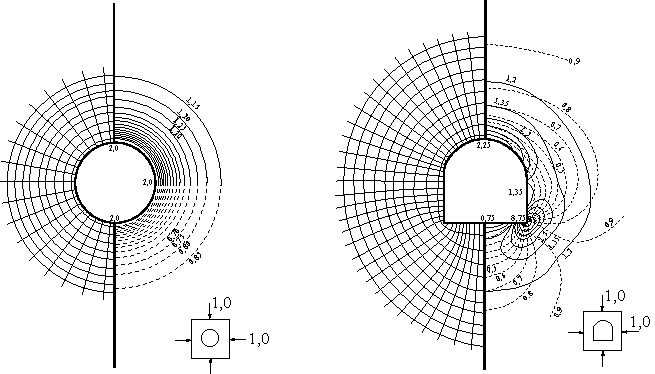
\includegraphics[scale = 1.3]{0419-trajetória das tensões principais.pdf}
	\end{center}
	\caption{\label{trajetorias_hoekbrown}Trajetória das tensões principais e linhas de isotensão, da maior e menor tensão principal, para seção circular (à esquerda) e ferradura (à direita) em condições geostáticas hidrostáticas (adaptado de: \citeonline[p. 469, 484]{Hoek1980})}
\end{figure}

\section{Influência da profundidade do túnel}

A profundidade do túnel está diretamente relacionada com o estado de tensões iniciais. Dados empíricos (\autoref{coeficiente_empuxo}a) sugerem que a tensão vertical pode ser estimada através da seguinte expressão \cite[p. 96]{Hoek1980}:

\begin{equation}
	\sigma_v(z=H)= \gamma_m H ,
\end{equation}

em que $\gamma_m$ é o peso específico do maciço e $H$ a profundidade do túnel. \citeonline{Hoek1980} reunem diversos dados que indicam que $\gamma_m$ (para maciços rochosos) situa-se na faixa de 20kN/m³ à 30kN/m³. Contudo, esses limites podem variar dependendo do banco de dados utilizado como, por exemplo, em \citeonline[p. 1030]{Martin2003}.

\begin{figure}[H]
	\begin{center}
		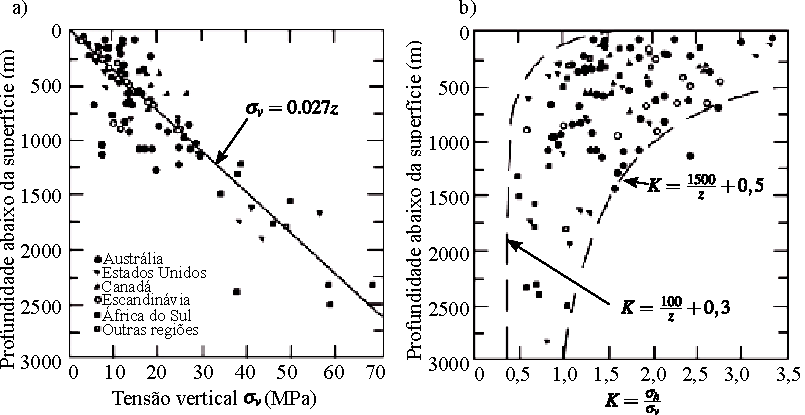
\includegraphics[scale = 1.0]{0420-tensoes verticais e coeficiente de empuxo k.pdf}
	\end{center}
	\caption{\label{coeficiente_empuxo}a) tensões verticais e b) razão entre a tensão horizontal e vertical (coeficiente de empuxo $K$)  (adaptado de: \citeonline[p. 99-100]{Hoek1980})}
\end{figure}

Como pode ser visto na \autoref{coeficiente_empuxo}b, há certa dispersão da tensão horizontal. Esse aspecto ainda hoje é objeto de estudo e uma boa revisão desses trabalhos pode ser obtido em \citeonline{Zhu2013}. Muitos desses trabalhos propõem equações simplificadas para obter o valor do coeficiente de empuxo $K$. Por exemplo, \citeonline[p. 32]{Sheorey1994} desenvolveu um modelo elasto-estático termal para as tensões na crosta da terra e obteve a seguinte equação simplificada que pode ser utilizada para estimar o coeficiente de empuxo $K$ em maciços rochosos:

\begin{equation}
	K = 0,25 + 7E_h(0,001+1/H).
\end{equation}

Sendo $H$ (m) a profundidade e $E_h$ (GPa) o módulo de deformação médio horizontal na parte superior da crosta terrestre. Contudo, como apontado por Sheorey, seu trabalho não explica a ocorrência de tensões verticais mais altas do que a profundidade indicaria ou o porquê de duas tensões horizontais raramente serem iguais. Segundo \citeonline[p. 67]{Hoek1998}, essas diferenças provavelmente se devem às características topográficas e geológicas locais, que não podem ser consideradas em um modelo de grande escala. Consequentemente, onde as tensões \textit{in situ} tendem a ter uma influência significativa no comportamento de aberturas subterrâneas é melhor medi-las \textit{in loco}.

Para túneis profundos, quando $H/D > 10$ , sendo $D$ o diâmetro equivalente da seção, é comum durante as análises, desprezar-se a variação da tensão vertical com a profundidade. Uma vez que, em túneis profundos, a variação de tensão ao longo do diâmetro da seção é irrelevante frente a magnitude da tensão na cota da profundidade, ou seja,

\begin{equation}
	\left|\Delta\sigma_v\right| = \left| \sigma_v(H+D/2)-\sigma_v(H-D/2)\right| = \left| \sigma_v(D) \right| <<  \left| \sigma_v(H)\right|.
\end{equation}

Esse princípio pode ser melhor entendido através da \autoref{tunel_profundo}.

\begin{figure}[H]
	\begin{center}
		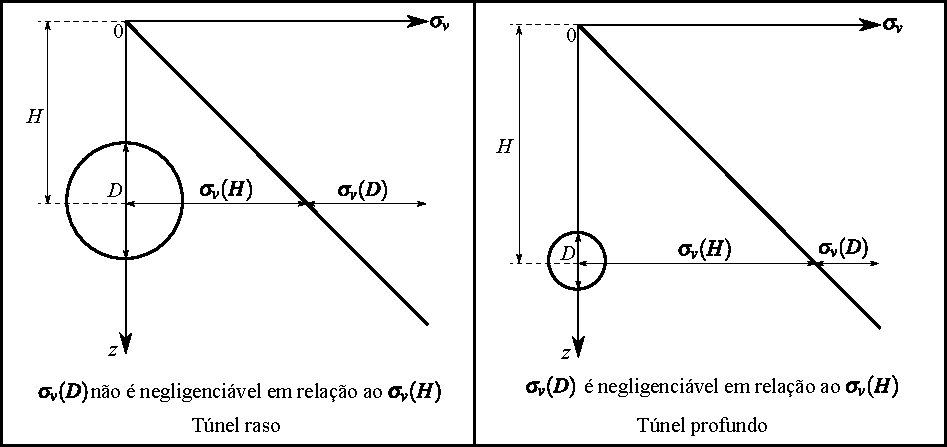
\includegraphics[scale = 1.0]{0421-tunelprofundo.pdf}
	\end{center}
	\caption{\label{tunel_profundo}Princípio para se desconsiderar a variação da tensão vertical na região próxima ao túnel  (adaptado de: \citeonline[p. 8]{Benamar1996})}
\end{figure}

De qualquer forma, conforme a \autoref{coeficiente_empuxo}, a consideração das tensões iniciais geostática hidrostática é apenas um caso específico de tensões \textit{in situ}, ou seja, quando $K=1$. A diferença entre as tensões verticais e horizontais afetam fortemente o campo de tensões e deformações após a escavação. Isso pode ser visto em análises elásticas com estado plano de deformações através, por exemplo, da comparação entre a \autoref{trajetorias_hoekbrown} e a \autoref{trajetorias_hoekbrown_aniso} obtidas por \citeonline{Hoek1980}.

\begin{figure}[H]
	\begin{center}
		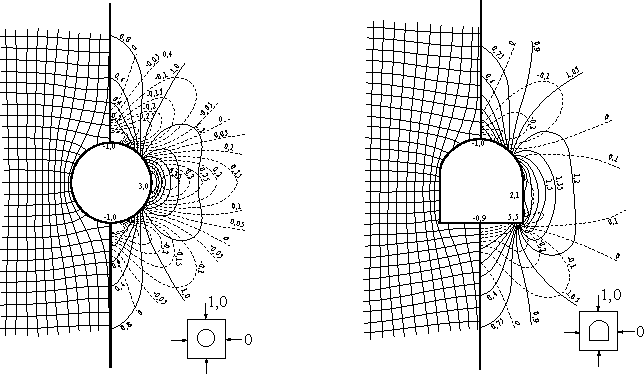
\includegraphics[scale = 1.3]{0422-trajetória das tensões principais_aniso.pdf}
	\end{center}
	\caption{\label{trajetorias_hoekbrown_aniso}Trajetória das tensões principais e linhas de isotensão da maior e menor tensão principal para seção circular (à esquerda) e ferradura (à direita) considerando $K=0$  (adaptado de: \citeonline[p. 468,483]{Hoek1980})}
\end{figure}

Além disso, quando o maciço apresenta um comportamento elastoplástico, a anisotropia das tensões \textit{in situ} afeta o formato da zona de plastificação. Isso pode ser visto no estudo de \citeonline{Detournay1988}. Utilizando soluções analíticas para seções circulares em um maciço elastoplástico com lei do comportamento de Mohr-Coulomb, esses autores apresentam um ábaco identificando os \textbf{modos de falha} (formas das zonas de plastificação) de acordo com o grau de anisotropia das tensões iniciais (\autoref{modos_falha}).

\begin{figure}[H]
	\begin{center}
		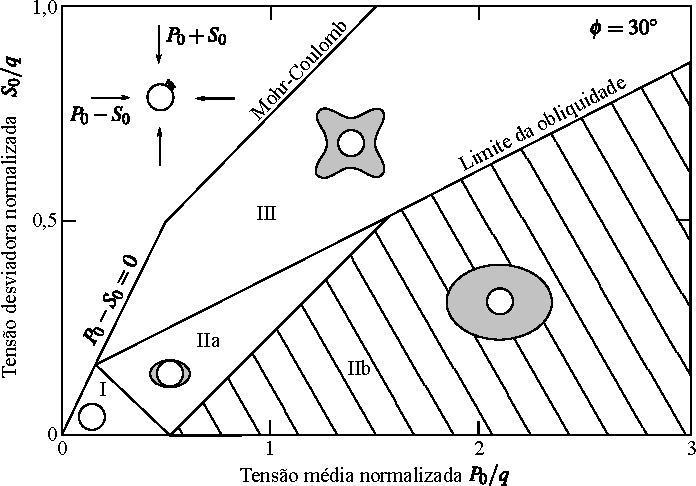
\includegraphics[scale = 1.0]{0423-modos_falha.pdf}
	\end{center}
	\caption{\label{modos_falha}Relação entre o estado de tensões iniciais e os modos de falha, onde $q_0$ é a resistência à compressão uniaxial do maciço (adaptado de: \citeonline[p.  121]{Detournay1988})}
\end{figure}

Como se pode ver na \autoref{modos_falha}, esses autores identificaram quatro zonas:

\begin{alineas}
	\item \textbf{região I}: a massa rochosa se comporta como um material elástico linear, ou seja, onde o estado de tensões não excedeu o critério de plasticidade em qualquer ponto;
	\item \textbf{região IIa}: a plastificação da rocha ao redor do túnel se estende em uma direção perpendicular a maior tensão principal de compressão, mas ainda não engloba completamente a seção do túnel;
	\item \textbf{região IIb}: a seção está completamente rodeada por uma zona de plastificação oval;
	\item \textbf{região III}: a zona de plastificação apresenta um formato de borboleta.
\end{alineas}

Além disso, quando há revestimento a anisotropia das tensões poderá ocasionar tração ou falha por compressão e cisalhamento na coroa ou nas paredes laterais do revestimento \cite{Brady2006}. Contudo, para uma situação em que $0 \leq K \leq 1$, em túneis profundos, a consideração de um estado geostático hidrostático ($K=1$) pode ser conservadora, para o dimensionamento do revestimento, como pode ser visto no estudo de \citeonline{Shrestha2015}.


\section{Influência da proximidade da superfície}

Quando o túnel está muito próximo da superfície, a região do maciço acima da seção não possui condições para formar a parte superior do arco transversal e desviar as tensões ao redor da cavidade. Isso faz com que essa parcela do maciço atue como sobrecarga sobre o revestimento. Dessa forma, o maciço no entorno de uma seção circular, por exemplo, não possui o campo de deslocamentos puramente radial. A rigor essa condição de túnel raso vai depender da capacidade resistente do maciço, contudo há na literatura indicações de que essa condição é atingida quando a altura de maciço sobre a coroa da seção transversal é menor que duas vezes o diâmetro \cite[p. 67]{Chapman2018}. Como consequência, a deformação da seção passa a apresentar três modos de deformações sobrepostos: uma convergência uniforme, uma distorção e translação vertical (\autoref{modos_deformacao}).

\begin{figure}[H]
	\begin{center}
		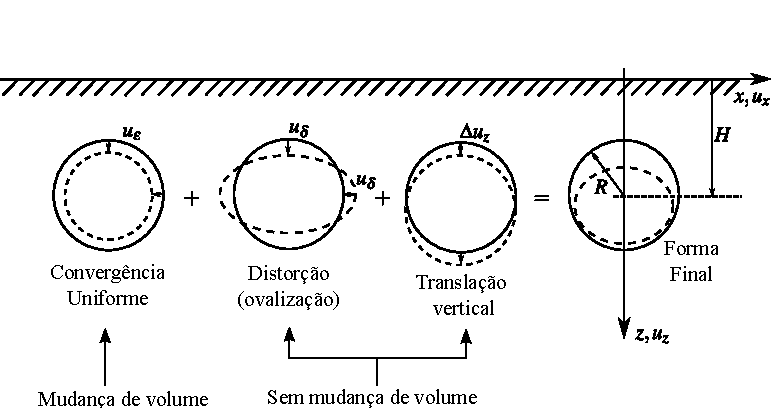
\includegraphics[scale = 1.0]{0424-modos_deformacao.pdf}
	\end{center}
	\caption{\label{modos_deformacao}Modos de deformações em túneis superficiais de seção circular (adaptado de: \citeonline[p. 4]{Pinto2014})}
\end{figure}

Quando o túnel apresenta um revestimento de concreto, por exemplo, o modo de deformação de distorção poderá induzir tensões de tração no interior do revestimento. Além disso, tão ou mais importante que a deformada da seção é o recalque induzido na superfície pelo processo de escavação. Conforme o túnel avança ele forma uma bacia de assentamento superficial que pode afetar as estruturas existentes (\autoref{bacia_assentamento}).

\begin{figure}[H]
	\begin{center}
		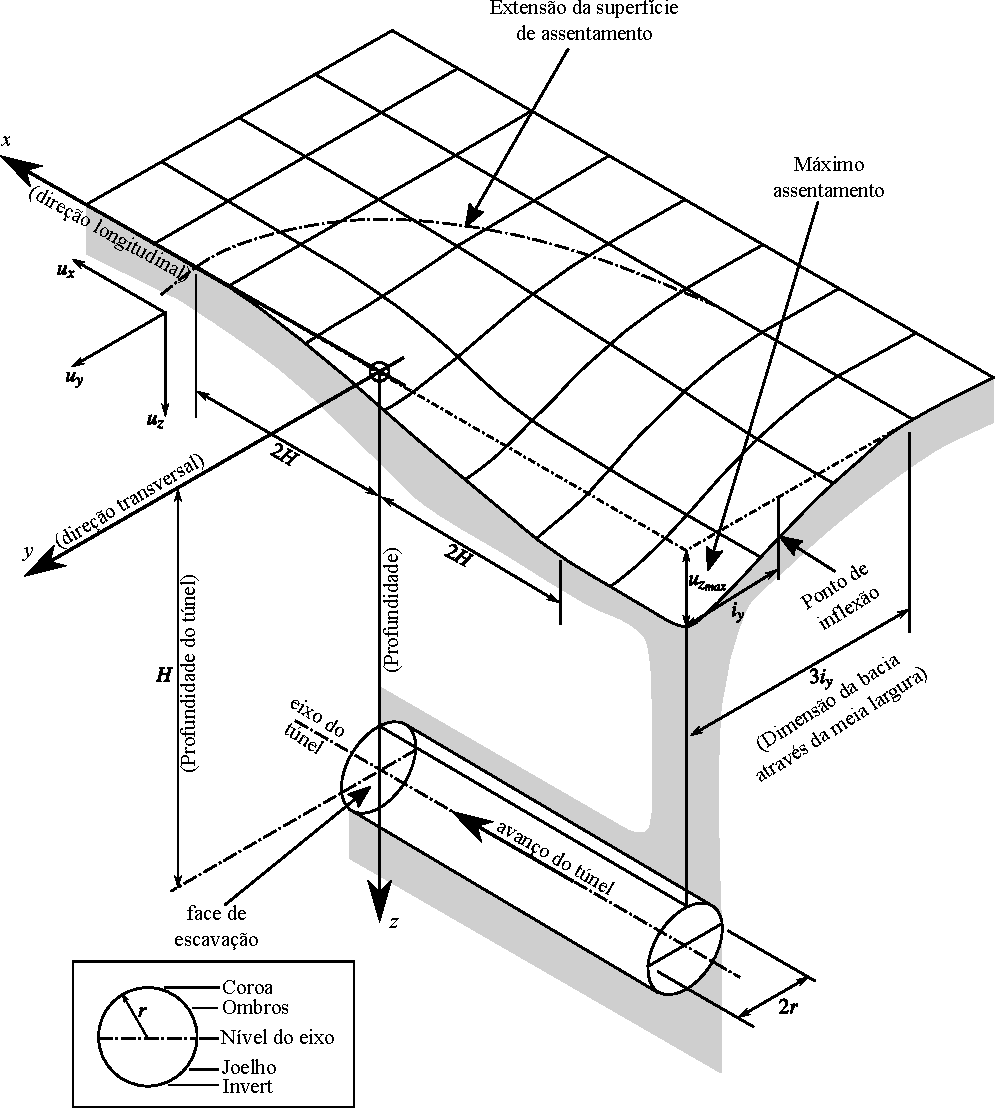
\includegraphics[scale = 1.0]{0425-bacia de assentamento.pdf}
	\end{center}
	\caption{\label{bacia_assentamento}Representação tridimensional da bacia de assentamento superficial durante a construção de um túnel superficial (adaptado de: \citeonline{Yeates1985} \textit{apud} \citeonline[p. 80]{Rankin2008})}
\end{figure}

Seguindo o trabalho de \citeonline{Martos1958} sobre assentamentos causados por minas \citeonline{Schmidt1969} e \citeonline{Peck1969}, e posteriormente muitos outros autores, mostraram que o perfil de assentamento no plano transversal pode muito bem ser descrito e ajustado, de forma empírica, através de uma curva de distribuição Gaussiana (\autoref{perfil_assentamento_transversal}).

\begin{figure}[H]
	\begin{center}
		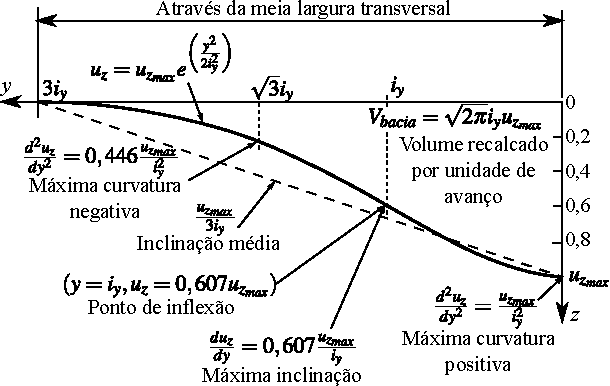
\includegraphics[scale = 1.0]{0426-perfil assentamento transversal.pdf}
	\end{center}
	\caption{\label{perfil_assentamento_transversal}Perfil idealizado de assentamento transversal com distribuição normal (adaptado de: \citeonline{OReilly1982} \textit{apud} \citeonline[p. 80]{Rankin2008})}
\end{figure}

Após \citeonline{Peck1969} propor sua forma empírica para descrever a bacia de assentamentos, adaptações dela e outros métodos semi-empíricos foram desenvolvidos com base em mais observações. Devido ao comportamento bastante específico relacionado a proximidade da superfície, os estudos sobre túneis se dividem em \textbf{túneis superficiais} e \textbf{túneis profundos}. Apesar da generalidade do modelo proposto na tese, a influência da superfície não será estudada no presente trabalho, que envolverá apenas túneis profundos, contudo, um bom resumo bibliográfico de soluções semi-empíricas pode ser encontrado em \citeonline{Zhou2018} e soluções numéricas na introdução de \citeonline{Panji2016}.

\section{Influência do revestimento e parâmetros adimensionais}

Dependendo da qualidade da rocha e das dimensões da abertura, muitos maciços conseguem desenvolver o arqueamento das tensões com pouca deformação ou ausência de plastificação. Isso caracteriza um maciço \textbf{autoportante} e, nesse caso, é necessário apenas um revestimento estético ou primário para evitar quedas localizadas. Contudo, se a redistribuição das tensões puder levar o maciço à plastificação ou deformações excessivas, nesse caso, é necessária a utilização de um \textbf{revestimento com função estrutural}. Dessa forma, a redistribuição das tensões para as zonas vizinhas no interior do maciço vai depender também dos deslocamentos permitidos por esse revestimento. Portanto, o estado de equilíbrio após a escavação não dependerá apenas das características do maciço, tensões iniciais, da geometria da seção e escavação, mas também do comportamento conjunto do maciço com esse revestimento. Consequentemente, o campo de tensões e deformações dependerão da rigidez relativa entre o maciço e o revestimento, da deformação do maciço no instante de colocação do revestimento, da distância não suportada em relação à frente de escavação e, quando há comportamentos diferidos no tempo, da velocidade de avanço da construção do túnel.

A \autoref{perfil_tensoes_verticais} ilustra, em um corte longitudinal, o perfil de convergências e tensões verticais sobre um túnel profundo revestido. À esquerda do ponto A o maciço encontra-se na zona não perturbada pela frente de escavação, mantendo, portanto, sua tensão vertical inicial $p_{\infty}$. Contudo, próximo à frente de escavação há um aumento das tensões verticais (entre os pontos A e B) devido ao arqueamento longitudinal das tensões próximo à face de escavação. No trecho não suportado $d_0$ as tensões verticais são nulas, uma vez que não há impedimento à deformação da seção. Todavia, a partir da ponta do revestimento (ponto D) há um acréscimo de tensões verticais (até o ponto E), novamente ocasionado pelo arqueamento longitudinal. Conforme a frente de escavação se afasta as tensões diminuem até atingirem um valor constante $p_{eq}$ (ponto F) e o perfil de convergências atinge um valor máximo e constante $Ueq$.

\begin{figure}[H]
	\begin{center}
		\includegraphics[scale = 1.0]{0427-perfil tensão vertical.pdf}
	\end{center}
	\caption{\label{perfil_tensoes_verticais}Perfil de tensões verticais e de convergências ao longo de uma linha longitudinal situada no teto do túnel (adaptado de: \citeonline{Eisenstein1984} \textit{apud} \citeonline[p. 41]{Couto2011})}
\end{figure}

O revestimento também possui interação com o comportamento diferido do maciço. O tempo entre ciclos de escavação-revestimento permitem que deformações viscosas ocorram durante a fase construtiva, ocasionando picos no perfil de convergência. Isso pode ser visto nas soluções numéricas axisimétricas obtidas por \citeonline{Bernaud1991} considerando uma lei elastoviscoplástica. A \autoref{perfil_convergencias_final_construção} mostra o efeito dessa interação no perfil de convergências. Pode-se ver que quanto maior a velocidade de escavação menores são os picos. E é possível notar também que a frequência desses picos está relacionada com o passo de escavação, que neste caso é de $1R$. Se o passo fosse menor, de $1/3R$, por exemplo, os picos seriam sensivelmente menores.

\begin{figure}[H]
	\begin{center}
		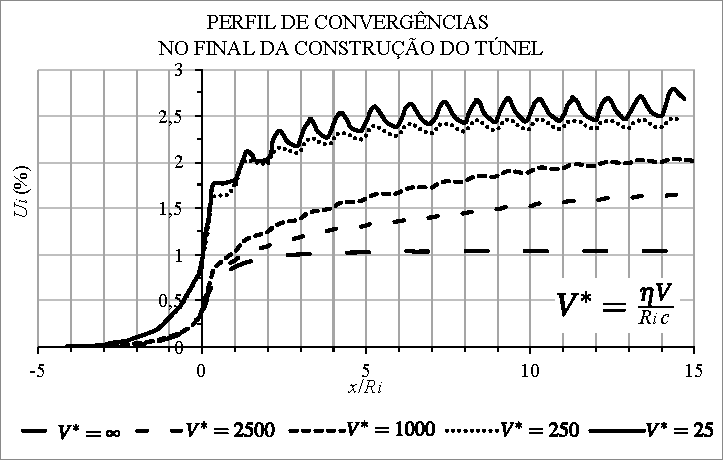
\includegraphics[scale = 1.0]{0428-perfil de convergencias no final da construção.pdf}
	\end{center}
	\caption{\label{perfil_convergencias_final_construção}Perfil de convergência em função da velocidade adimensional de avanço no final da construção do túnel (adaptado de: \citeonline[p. 214]{Bernaud1991})}
\end{figure}

Contudo, os efeitos viscosos continuam mesmo após a construção do túnel. Com o tempo a convergência da seção vai aumentando e a pressão no revestimento diminuindo. Além disso, quanto mais rápido for o ciclo de escavação-revestimento, maior será a diferença entre a convergência no final da construção e após estabilizado os efeitos viscosos no longo prazo. Isso pode ser visto comparando-se a \autoref{perfil_convergencias_final_construção} com a \autoref{perfil_convergencias_apos_efeitos_viscosos}.

\begin{figure}[H]
	\begin{center}
		\includegraphics[scale = 1.0]{0429-perfil de convergencias após efeitos viscosos.pdf}
	\end{center}
	\caption{\label{perfil_convergencias_apos_efeitos_viscosos}Perfil de convergência em função da velocidade de construção admensionalizada no final da construção do túnel (adaptado de: \citeonline[p. 214]{Bernaud1991})}
\end{figure}

Um aspecto importante derivado das soluções analíticas é a identificação de parâmetros adimensionais que governam a problemática de túneis e permitem extrapolar os valores de uma análise para outra adimensionalmente equivalente. Dado essa generalidade são parâmetros muito utilizados para apresentação de resultados, como os que constam na \autoref{perfil_convergencias_final_construção} e \autoref{perfil_convergencias_apos_efeitos_viscosos}.

Segundo \citeonline[p. 5]{Bernaud1994}, nas soluções analíticas em estado plano de deformações, considerando tanto o maciço quanto o revestimento com leis constitutivas elásticas, obtêm-se os seguintes parâmetros adimensionais:

\begin{equation}
	p_\infty^* = \frac{p_\infty}{E},~~~ K_r^* = \frac{K_r}{E},~~~ d_0^* = \frac{d_0}{R} 
\end{equation}

em que $E$ é o módulo de elasticidade do maciço, $p_\infty$ a pressão geostática hidrostástica, $K_r$ a rigidez equivalente do revestimento, $d_0$ a distância não revestida logo atrás da frente de escavação e $R$ o raio externo da abertura circular do túnel. Quando o maciço possuí lei constitutiva elastoplástica de Tresca ou von-Mises, acrescenta-se mais um parâmetro adimensional:

\begin{equation}
	c^* = \frac{c}{E} 
\end{equation}

sendo $c$ a coesão do maciço. Além disso, quando o túnel se encontra imerso em um meio elastoviscoplástico perfeito com modelo de Perzyna, tem-se cinco parâmetros adimensionais, que são \cite[p. 198]{Bernaud1991}:

\begin{equation}
	E^* = \frac{E}{c},~~~ p_\infty^* = \frac{p_\infty}{c},~~~ K_r^* = \frac{K_r}{c},~~~ d_0^* = \frac{d_0}{R},~~~ V^*=\frac{\eta V}{Rc}
\end{equation}

em que $\eta$ é a constante de viscosidade dinâmica (em unidade de tensão vezes tempo) e $V$ a velocidade de avanço do túnel.

Contudo, a principal dificuldade na determinação do estado de equilíbrio de um túnel revestido está no fato de que o maciço já possui uma convergência $U_0$ no instante de instalação do revestimento. E essa convergência é dependente da interação entre o maciço e o revestimento que já foi aplicado. Uma forma de lidar com essa complexidade é através do método Convergência-Confinamento (também conhecido como o método das Curvas Características).

\section{Método convergência-confinamento}

Muitos autores propuseram contribuições para essa abordagem como \citeonline{Fenner1938}, \citeonline{Pacher1964}, \citeonline{Panet1974} e \citeonline{Bernaud1992}. Esse método consiste em desacoplar o problema da interação entre o maciço e o revestimento utilizando os conceitos de curva de convergência do maciço e de curva de confinamento do revestimento. 

A \textbf{curva de convergência do maciço} (CV) é obtida graficando-se a convergência $U_i$ em função de uma pressão interna fictícia $p_i$ atuante no interior da cavidade, partindo essa pressão da tensão inicial geostática-hidrostática $p_\infty$ até zero. Essa curva de convergência é independente do suporte e carrega consigo o comportamento do maciço frente a uma descompressão simulada pela variação de $p_i$ (ver curva azul na \autoref{metodo cv-cf}). Quando o maciço possui um comportamento elastoplástico, a curva apresenta um trecho linear elástico até que a descompressão atinge um valor limite $p_{lim}$, sendo a partir daí um trecho não-linear. Resumo de soluções analíticas para essa curva, considerando estado plano de deformações, seção circular e tensões iniciais geostáticas-hidrostáticas, pode ser encontrado, por exemplo, em \citeonline{Brown1983} e \citeonline{Corbeta1990}.

A aplicação desse método está no fato de que é possível também construir uma curva análoga referente ao suporte, chamada de \textbf{curva de confinamento do revestimento} (CF) (ver curva vermelha na \autoref{metodo cv-cf}) cuja intersecção com a curva de convergência fornecerá o ponto de equilíbrio $(p_{eq},U_{eq})$ que é a solução do problema da interação entre o maciço e o revestimento. Tal como utilizado por \citeonline[p. 29]{Panet1995} soluções analíticas para tubos espessos ou casca cilíndrica, mesmo em elasticidade, podem corresponder como uma primeira aproximação da curva de confinamento para um dado revestimento.

Apesar do comportamento da curva de confinamento depender exclusivamente da lei constitutiva do revestimento, a convergência inicial $U_0$, a partir da qual essa curva inicia, vai depender da interação entre o maciço e do revestimento que foi anteriormente instalado, uma vez que a seção do túnel, afastada de $d_0$ da face de escavação, já possui essa convergência durante o avanço construtivo do túnel.

\begin{figure}[H]
	\begin{center}
		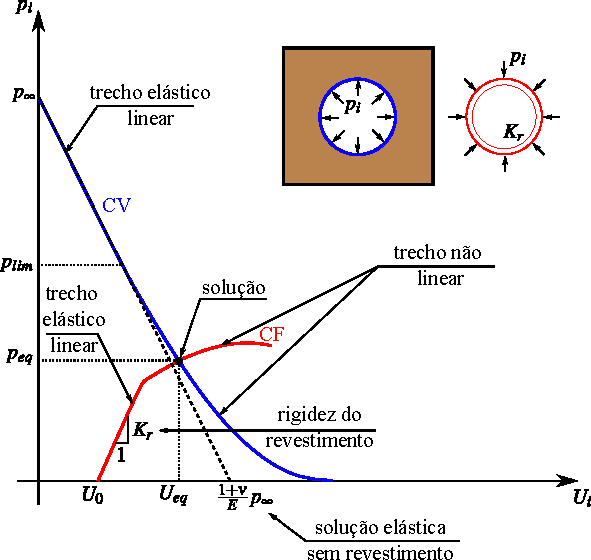
\includegraphics[scale = 1.0]{0430-metodo convergencia-confinamento.pdf}
	\end{center}
	\caption{\label{metodo cv-cf}Método da Convergência-Confinamento (adaptado de: \citeonline[p. 6]{Bernaud1994})}
\end{figure}

As curvas de convergência (CV) e de confinamento (CF) podem ser obtidas tanto de soluções analíticas como numéricas em estado plano de deformações, sendo que no caso numérico podem considerar leis mais complexas de comportamento do maciço. Contudo, a determinação de $U_0$ só pode ser feita através de um método que considere a completa interação entre o maciço e o revestimento, como análises tridimensionais, axissimétricas ou ainda medidas \textit{in situ}.

Existem métodos simplificados que se diferenciam justamente nas propostas de $U_0$ através de estudos, por exemplo, em axissimetria. Nesse aspecto, \citeonline{Bernaud1992}, mostraram que o método CV-CF proposto até então, estava em desfavor da segurança, pois desconsiderava a rigidez do revestimento na determinação de $U_0$   (\autoref{metodo NIM}), o que significa que o método CV-CF não considerava de forma correta a interação entre o maciço e o revestimento.

\begin{figure}[H]
	\begin{center}
		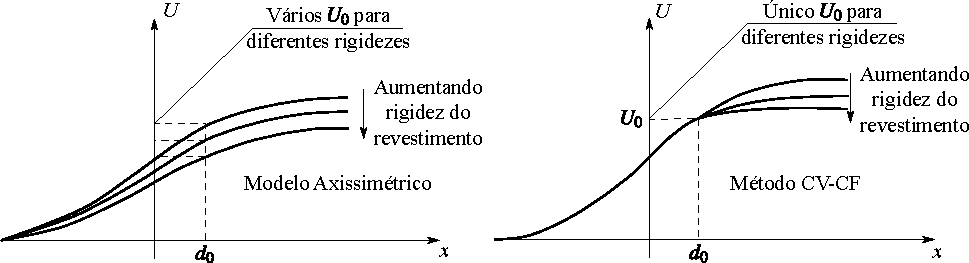
\includegraphics[scale = 1.0]{0431-influencia da rigidez do suporte no perfil de convergencias.pdf}
	\end{center}
	\caption{\label{metodo NIM}Influência da rigidez do revestimento no perfil de convergências do túnel e no parâmetro $U_0$ (adaptado de: \citeonline[p. 13]{Bernaud1992})}
\end{figure}

Em vista disso, esses autores propuseram uma correção ao método Convergência-Confinamento criando o \textit{New Implicit Method} (NIM). Um método implícito, pois $U_0$ depende tanto da rigidez do revestimento quanto da convergência ao equilíbrio (que se quer determinar). Esse método foi desenvolvido para leis de comportamento do maciço em elasticidade, plasticidade e viscoplasticidade, conforme \citeonline{Bernaud1992} e \citeonline{Bernaud1994}.